\documentclass[aps,secnumarabic,amsmath,amssymb,10pt,superscriptaddress]{revtex4}
\usepackage{amsmath}
\usepackage{amssymb}
\usepackage{amsfonts}
\usepackage{color}
\usepackage{graphics}
\usepackage[pdftex]{graphicx}
\usepackage[utf8x]{inputenc}
\usepackage[colorlinks=true]{hyperref}
\usepackage{listings}
\usepackage{braket}
\usepackage{xcolor}
\newcommand\jmh[1]{{\color{magenta} #1}}

\newcommand{\ud}{\mathrm{d}}
\newcommand{\ue}{\mathrm{e}}
\newcommand{\ui}{\mathrm{i}}
\newcommand{\res}{\mathrm{Res}}
\newcommand{\Tr}{\mathrm{Tr}}
\newcommand{\dsum}{\displaystyle\sum}
\newcommand{\dprod}{\displaystyle\prod}
\newcommand{\dlim}{\dispqlaystyle\lim}
\newcommand{\dint}{\displaystyle\int}
\newcommand{\fsno}[1]{{\!\not\!{#1}}}
\newcommand{\texp}[2]{\ensuremath{{#1}\times10^{#2}}}
\newcommand{\dexp}[2]{\ensuremath{{#1}\cdot10^{#2}}}
\newcommand{\eval}[2]{{\left.{#1}\right|_{#2}}}
\newcommand{\paren}[1]{{\left({#1}\right)}}
\newcommand{\lparen}[1]{{\left({#1}\right.}}
\newcommand{\rparen}[1]{{\left.{#1}\right)}}
\newcommand{\abs}[1]{{\left|{#1}\right|}}
\newcommand{\sqr}[1]{{\left[{#1}\right]}}
\newcommand{\crly}[1]{{\left\{{#1}\right\}}}
\newcommand{\angl}[1]{{\left\langle{#1}\right\rangle}}
\newcommand{\tpdiff}[4][{}]{{\paren{\frac{\partial^{#1} {#2}}{\partial {#3}{}^{#1}}}_{#4}}}
\newcommand{\tpsdiff}[4][{}]{{\paren{\frac{\partial^{#1}}{\partial {#3}{}^{#1}}{#2}}_{#4}}}
\newcommand{\pdiff}[3][{}]{{\frac{\partial^{#1} {#2}}{\partial {#3}{}^{#1}}}}
\newcommand{\diff}[3][{}]{{\frac{\ud^{#1} {#2}}{\ud {#3}{}^{#1}}}}
\newcommand{\psdiff}[3][{}]{{\frac{\partial^{#1}}{\partial {#3}{}^{#1}} {#2}}}
\newcommand{\sdiff}[3][{}]{{\frac{\ud^{#1}}{\ud {#3}{}^{#1}} {#2}}}
\newcommand{\tpddiff}[4][{}]{{\left(\dfrac{\partial^{#1} {#2}}{\partial {#3}{}^{#1}}\right)_{#4}}}
\newcommand{\tpsddiff}[4][{}]{{\paren{\dfrac{\partial^{#1}}{\partial {#3}{}^{#1}}{#2}}_{#4}}}
\newcommand{\pddiff}[3][{}]{{\dfrac{\partial^{#1} {#2}}{\partial {#3}{}^{#1}}}}
\newcommand{\ddiff}[3][{}]{{\dfrac{\ud^{#1} {#2}}{\ud {#3}{}^{#1}}}}
\newcommand{\psddiff}[3][{}]{{\frac{\partial^{#1}}{\partial{}^{#1} {#3}} {#2}}}
\newcommand{\sddiff}[3][{}]{{\frac{\ud^{#1}}{\ud {#3}{}^{#1}} {#2}}}
\newcommand{\eff}{ef\! f}

\newcommand{\todo}[1]{}
\newcommand{\Na}{\mathrm{Na}}
\newcommand{\Cs}{\mathrm{Cs}}

\newcommand{\harvardphysics}{\affiliation{Department of Physics, Harvard University, Cambridge, Massachusetts 02138, USA}}
\newcommand{\harvardccb}{\affiliation{Department of Chemistry and Chemical Biology, Harvard University, Cambridge, Massachusetts 02138, USA}}
\newcommand{\cua}{\affiliation{Harvard-MIT Center for Ultracold Atoms, Cambridge, Massachusetts 02138, USA}}
\newcommand{\gradstudent}{
  \harvardphysics
  \harvardccb
  \cua
}

% Add S1 to bibliography
\bibliographystyle{apsrev4-2}
\renewcommand*{\citenumfont}[1]{S#1}
\renewcommand*{\bibnumfmt}[1]{[S#1]}

% Add S to labels
\setcounter{table}{0}
\renewcommand{\thetable}{S\arabic{table}}%
\setcounter{figure}{0}
\renewcommand{\thefigure}{S\arabic{figure}}%
\renewcommand{\thepage}{S\arabic{page}}
\renewcommand{\thesection}{S\arabic{section}}
\renewcommand{\theequation}{S.\arabic{equation}}

\ifpdf
% Ensure reproducible output
\pdfinfoomitdate=1
\pdfsuppressptexinfo=-1
\pdftrailerid{}
\hypersetup{
  pdfcreator={},
  pdfproducer={}
}
\fi

\begin{document}
\title{Two photon coupling to atomic relative motional continuum}

\maketitle

As the reverse process of the Raman transition that forms the molecule,
the ground molecular state can be driven to the atomic state as well.
If the energy for such atomic state is above the trap depth of the tweezer,
this can couple the molecule to a continuum and therefore lead to loss.
Physically, this loss corresponds to a photodissociation process
where the two atoms flies apart with high kinetic energy.

The photodissociation rate is determined by the Fermi's golden rule,
\[
  \Gamma=2\pi\Omega_{if}^2\ \rho_f
\]
where $\Omega_{if}$ is the matrix element between the initial and final state
and $\rho_f$ is the density of state near the final state.
We calculate this by first discretizing the continuum and the rate becomes
\[
  \Gamma=2\pi\frac{{\Omega'_{if}}^2}{\delta}
\]
where $\Omega'_{if}$ is the Rabi frequency between the initial and final state
and $\delta$ is the spacing between the discretized final states.

The Rabi frequency $\Omega'_{if}$ is proportional to the square root of FCF,
which we calculate for the atomic ground motional states by exactly diagonalization
of the atomic wavefunction.
However, due to the high energy~($\approx\!1~\mathrm{GHz}$) of the final state,
calculating FCF for the target state using this method requires an unrealiztic number of
states to be included.
Instead, we approximate it using the results for the atomic ground state
by assuming the FCF to be proportional to the probability density of non-interacting
atomic wavefunction at zero relative distance so that,
\[
  \Omega'_{if}=\Omega_0\frac{\psi_f\paren{r_{rel}=0}}{\psi_0\paren{r_{rel}=0}}
\]
where $\Omega_0$ is the Rabi frequency between the excited state and
the atomic motional ground state and $\psi_f$ and $\psi_0$ are the
wavefunctions of the final and ground motional atomic state without the molecular potential.
This approximation is justifed because,
\begin{enumerate}
\item The molecular potential is short ranged and the excited molecular state is small.
\item Only the final atomic wavefunction within the molecular potential contributes to the FCF.
  For relatively low motional energy
  this wavefunction is proportional to the value of the wavefunction at
  the edge of the molecular potential which is well approximated by
  the atomic wavefunction without the molecular potential.
\end{enumerate}
This approximation remains valid until the de Broglie wavelength for the atomic state
is comparable to the size of the molecular potential which corresponds to
a motional energy of $\approx\!40~\mathrm{GHz}$.
For atomic motional ground state, we have,
\begin{align*}
  \psi_0\paren{r_{rel}=0}=&\prod_{i=1}^{3}\paren{\frac{\mu\omega_i}{\pi}}^{1/4}\\
  =&\paren{\frac{\mu^3\omega_1\omega_2\omega_3}{\pi^3}}^{1/4}
\end{align*}
where $\mu$ is the reduced mass $\mu\equiv m_\Na m_\Cs/\paren{m_\Na+m_\Cs}$,
and $\omega_i$'s are the relative trapping frequencies along the three trap axis.
We discretize the continuum state by adding an infinitely deep spherical potential well
of radius $R$ around the center. The radial wavefunctions of the eigenstates
within the well with quantum number $n=1,2,\dots$ is,
\begin{align*}
  \psi_n=&\frac{1}{\sqrt{4\pi}r_{rel}}\sqrt{\frac{2}{R}}\sin\paren{\frac{\pi nr_{rel}}{R}}
\end{align*}
and the corresponding energy,
\begin{align*}
  E_n=&\frac{\pi^2n^2}{2\mu R^2}
\end{align*}
The energy gap between neighboring states is
\begin{align*}
  \delta_n\approx&\frac{\pi^2n}{\mu R^2}
\end{align*}
and the wavefunction value at $r_{rel}=0$ is,
\begin{align*}
  \psi_n\paren{r_{rel}=0}=&\sqrt{\frac{1}{2\pi R}}\left.\frac{\ud}{\ud r_{rel}}\sin\paren{\frac{\pi nr_{rel}}{R}}\right|_{r_{rel}=0}\\
  =&\frac{\pi n}{\sqrt{2\pi R}R}
\end{align*}
Substituting into $\Gamma$ and taking the limit of $R\rightarrow\infty$ we have
\begin{align*}
  \Gamma=&2\pi\frac{\Omega_0^2}{\delta}\frac{\psi_f^2\paren{r_{rel}=0}}{\psi_0^2\paren{r_{rel}=0}}\\
  =&\Omega_0^2\frac{n}{R}\sqrt{\frac{\pi^3}{\mu\omega_1\omega_2\omega_3}}=\Omega_0^2\sqrt{\frac{2\pi E}{\omega_1\omega_2\omega_3}}
\end{align*}

\begin{figure}[ht!]
  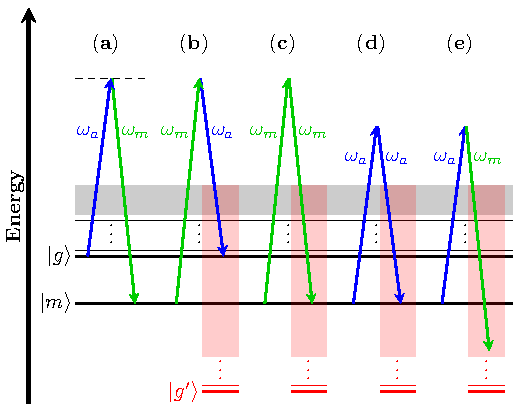
\includegraphics[width=0.6\textwidth]{imgs/pa_two_photon_down_raman.pdf}
  \caption{
    Effect of two-photon coupling to atomic contimuum on molecular state.
    (a) Raman transition from the atomic ground state $|g\rangle$
    to the molecular bound state $|m\rangle$ using two Raman beams with frequencies
    $\omega_1$ and $\omega_2$.
    (b-e) Two photon transitions starting from the molecular state $|m\rangle$
    with different frequency combinations without additional atomic spin states.
    (b) This is the reverse Raman transition and reaches the initial atomic state.
    (c,d) The frequency pairs couples back to $|m\rangle$.
    (e) This couples to an energy below $|m\rangle$.
    Note that none of the two-photon transitions from $|m\rangle$ in (b-e) ends up in
    the atomic motional continuum (gray) for the spin state $|g\rangle$.
    However, it is coupled to the motional continuum
    for the spin state with lower energy $|g'\rangle$
    and may be affected by the corresponding dissociative scattering.
    \label{f-raman-continuum}}
\end{figure}

As shown in Fig.~\ref{f-raman-continuum},
since we only have the two Raman frequencies in the experiment,
the energy of the final state is never higher than that of the initial atomic state
and well below the corresponding trap depth.
Therefore, in order to couple to the continuum,
the final state must belong to a different atomic spin state with lower energy.
For our initial spin state of $\Na(2,2),\Cs(3,3)$,
the only candidate for such state is therefore $\Na(1,1),\Cs(3,3)$,
which is lower in energy by $E_{\mathrm{HF}}\approx1.77~\mathrm{GHz}$.
Due to the conservation of $m_f$, this coupling is forbidden if the tweezer is $\pi$-polarized.
Therefore, such coupling can only be caused by impurity in the tweezer polarization.
Using a previously measured tweezer polarization of $C=0.0545$,
where $\mathbf{C}\equiv\abs{\mathrm{Im}\paren{\mathbf{\varepsilon}\times\mathbf{\varepsilon}^*}}$
and $\mathbf{\varepsilon}$ is the polarization vector,
we estimated the Raman Rabi frequency between the molecular state and the $\Na(1,1),\Cs(3,3)$
ground state to be $\Omega_0\approx2\pi500~\mathrm{Hz}$.
Combining the 4 different pathways in Fig.~\ref{f-raman-continuum}(b-e),
the total scattering expected is,
\begin{align*}
  \Gamma=&\Omega_0^2\sqrt{\frac{2\pi}{\omega_1\omega_2\omega_3}}
           \paren{\sqrt{E_{\mathrm{HF}}}+4\sqrt{E_{\mathrm{HF}}-E_b}+\sqrt{E_{\mathrm{HF}}-2E_b}}\\
  \approx&2\pi\times200~\mathrm{Hz}
\end{align*}
where $E_b$ is the binding energy of the molecule.
The order-of-magnitude agreement between this rough estimate and the observed loss rate
of $2\pi\times800~\mathrm{Hz}$ suggests that this loss mechanism
could potentially explain the loss we observe given the correct tweezer polarization.

\end{document}
